% First TeX Draft für Fabi's Diss. Adapted from Tobi's texfile
\documentclass[twoside,10pt,openright]{scrbook} % right-side equation numbering, 10 point font, print two-sided, chapterbegin on the right

\KOMAoptions{BCOR=16mm,  	%
 	     DIV=12,		%
	     twocolumn=false, 	%
	     paper=A4, 		%
	     draft=false,	%
	     titlepage=true,	%
	     toc=listof,	%
	     headsepline=true,	%
	     footsepline=false,
	     toc=bibliography,
	     numbers=noendperiod}

\usepackage[default]{lato}
\usepackage{amsxtra}     % Use various AMS packages
\usepackage{amsthm}
\usepackage{amssymb}
\usepackage{amsfonts}
\usepackage{mathpazo}
\usepackage{graphicx}    % Add some packages for figures. Read epslatex.pdf on ctan.tug.org
\usepackage{caption}    % Add some packages for figures. Read epslatex.pdf on ctan.tug.org
\usepackage{rotating}
\usepackage{color}
\usepackage{epsfig}
\usepackage{subfigure}   % To make subfigures. Read subfigure.pdf on ctan.tug.org
\usepackage{verbatim}
\usepackage{natbib}      % Allows you to use BibTeX
\usepackage{setspace}    % Allows you to specify the line spacing
\usepackage{parskip}	 % no indent
\usepackage{fancyhdr}
\usepackage{tabularx}
\usepackage{nomencl}
\usepackage{lscape}
\usepackage[utf8]{inputenc} % to be sure
\usepackage{csquotes}
\usepackage{index}
\usepackage{float}
\usepackage{pdfpages}
\usepackage{textcomp} % \textcelsius
\usepackage{nth}
\usepackage{enumerate}
\usepackage{enumitem}
\usepackage{cclicenses}
\usepackage{wrapfig}
\usepackage{minted}
\usepackage{hanging}
\usepackage{bbding}
\usepackage{microtype}
%\usepackage[section]{placeins} this was to force figures to section. in the end maybe
\usepackage{placeins}
\usepackage[usenames,dvipsnames]{xcolor}
\usepackage[toc,page]{appendix}
\usepackage{perpage} %the perpage package
\MakePerPage{footnote} %the perpage package command
\usepackage{float}

\usepackage[bookmarks,colorlinks,citecolor=MidnightBlue,urlcolor=MidnightBlue,linkcolor=MidnightBlue,hypertexnames=false]{hyperref}
%\usepackage[bookmarks,colorlinks,citecolor=Black,urlcolor=Black,linkcolor=Black,hypertexnames=false]{hyperref}

\newcommand{\HRule}{\rule{\linewidth}{0.5mm}}
%\renewcommand*{\thefootnote}{\fnsymbol{footnote}}
%\newcommand\HUGE{\@setfontsize\Huge{38}{47}} 

\newcommand{\figs}{../habil/img}

%\doublespacing %gonehalfspacing for 1.5 spacing, \doublespacing for 2.0 spacing.
\onehalfspacing

\author{Fabien Maussion}
\title{Numerical modelling of \\ global glacier change}
\subtitle{}
\date{2021}

\makeatletter
\def\thickhrulefill{\leavevmode \leaders \hrule height 1pt\hfill \kern \z@}
\renewcommand{\maketitle}{\begin{titlepage}%
  
	\begin{center}
		% Upper part of the page
	  	\vspace*{0cm}
		\Huge \bfseries \MakeUppercase{\@title} \mdseries \\[1.5cm]
				
		\Large \MakeUppercase{Habilitation thesis} \\	[1cm]		
		\Large Fabien Maussion \\	[0.1cm]		
		\large 2021 \\ [4.5cm]

		\begin{figure}[h!]
		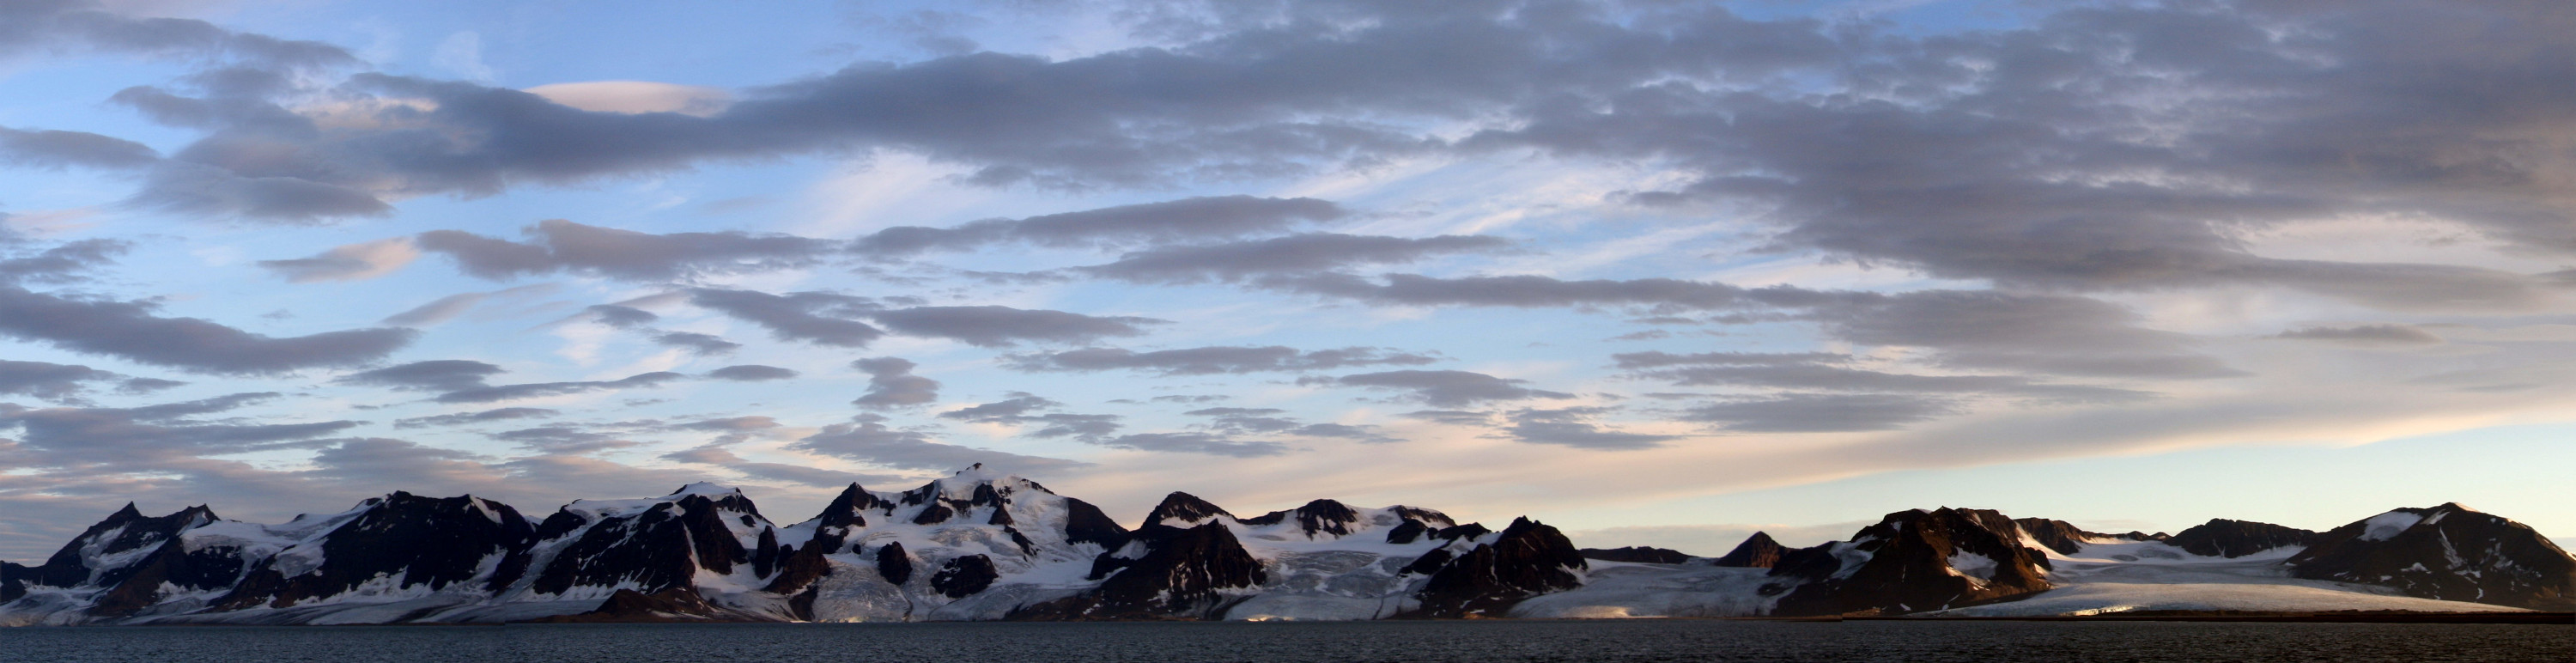
\includegraphics[width=\textwidth ,angle=0]{\figs/title_pic.jpeg} \\ [3cm]
		\end{figure}

		\large Submitted to the Faculty of Geo- and Atmospheric Sciences \\ at the University of Innsbruck, Austria.
	\end{center}
        %\large Institut für Ökologie \\[0.2cm]
        %\large Fachgebiet Klimatologie \\[1.2cm]  
		%\large Dr. rer. nat. \\[1.2cm]
  \end{titlepage}%
  \setcounter{footnote}{0}%
}
\makeatother


%----------------------------------------------------
% Chapter  style
%----------------------------------------------------
\makeatletter
\def\@makechapterhead#1{%
  \vspace*{50\p@}%
  {\parindent \z@ \raggedleft \normalfont
    \ifnum \c@secnumdepth >\m@ne
      \if@mainmatter
      \Large \@chapapp\space \Huge\thechapter
        \par\nobreak
        \vskip 40\p@
      \fi
    \fi
    \interlinepenalty\@M
    \hrule
    \vspace*{12\p@}%
    \huge #1\par\nobreak
    \par
    \vspace*{20\p@}%
    \hrule
    \vskip 50\p@
  }}
\def\@schapter#1{\if@twocolumn
                   \@topnewpage[\@makeschapterhead{#1}]%
                 \else
                   \@makeschapterhead{#1}%
                   \@afterheading
                 \fi}
\def\@makeschapterhead#1{%
  \vspace*{50\p@}%
  {\parindent \z@ \raggedleft
    \normalfont
    \interlinepenalty\@M
    \hrule
    \vspace*{6\p@}%
    \Large #1\par\nobreak
    \par
    \vspace*{15\p@}%
    \hrule
    \vskip 40\p@
  }}
\makeatother

%-----------------------------------
% Header top/bottom
%-----------------------------------
\pagestyle{fancy}

%\renewcommand{\chaptermark}[1]{%
%\markboth{\MakeUppercase{%
%\chaptername}\ \thechapter.%
%\ #1}{}}
%\renewcommand{\chaptermark}[1]{\markboth{{\thechapter} #1}{}}
%\renewcommand{\sectionmark}[1]{\markright{{\thesection} #1}{}}

\renewcommand{\headrulewidth}{0pt}% Remove header rule
\fancyhead{}% Remove all header contents

%\definecolor{cadet}{RGB}{54,100,139}
%\definecolor{cadet}{RGB}{96,123,139}
%\definecolor{cadet}{RGB}{67,84,112}
%\fancyhead[]{}
%\fancyhead[RO]{{\rightmark}} % clear all header fields
%\fancyhead[LO]{}
%\fancyhead[LE]{{\leftmark}}
%\fancyhead[RE]{}
\fancyfoot{} % clear all footer fields
\fancyfoot[LE,RO]{\thepage}
\fancyfoot[LO,RE]{}
%\renewcommand{\headrulewidth}{0.4pt}
%\renewcommand{\footrulewidth}{0.4pt}




%----------------------------------
% Textauszeichnungen
%----------------------------------
\addtokomafont{captionlabel}{\footnotesize\bfseries}
\addtokomafont{caption}{\footnotesize}
\addtokomafont{section}{\Large}
\addtokomafont{subsection}{}
\addtokomafont{subsubsection}{}

\begin{document}

% Titleblatt einfügen
\maketitle

\frontmatter
\addchap{Preface}


This habilitation thesis consists of 13 peer reviewed publications completed
between 2015 and 2020. It also contains two short, previously unpublished chapters
introducing what I believe to be my most important contributions to the field of
large-scale glaciology to date: (i) the \href{https://oggm.org}{Open Global Glacier Model (OGGM)},
an open-source glacier evolution model, and (ii) \href{https://edu.oggm.org}{OGGM-Edu},
a collaborative educational website about glaciers. All papers, web platforms
and software presented here were prepared while I was working at the University of Innsbruck.

This thesis addresses several aspects of the numerical modelling of glacier change,
at various spatial (glacier to global) and temporal (annual to centennial) scales. Thanks to
the projects I had the chance to contribute to, it also develops some aspects of observational
glaciology and meteorology. However, the main bulk of this work is focussing on the central
topic of this thesis: \textbf{the development of modern numerical methods to (i) estimate the ice
thickness of mountain glaciers and their volume, (ii) compute their mass balance and (iii)
simulate their evolution under climate change}.

A further important theme that is developed in this thesis is the topic of \textbf{open science}.
Because of my personal conviction that all scientific results should be openly available, I have
spent a lot of thought and energy on developing methods and workflows that enable a more open,
accessible, documented, and reproducible scientific practice. Many of these ideas are not from my
own invention, but are workflows that I borrowed and adapted from the open-source software
development community.

All the work presented here is the result of numerous collaborations, within the University of Innsbruck,
but also originating from a wider network of collaborators and from international working groups.
Five of these papers arose from my contributions
to the doctoral studies of Beatriz Recinos and Julia Eis (University of Bremen), Ben Pelto (University of
Northern British Columbia), Stephan Galos (University of Innsbruck) and the master thesis of
Tobias Zolles (University of Innsbruck). \\ [0.8cm]

\textit{This thesis is also available as a website:}
\href{https://fabienmaussion.info/habil2.0}{www.fabienmaussion.info/habil2.0} \\
\textit{The content is strictly the same - readers are free to choose which format suits them better!}

\section*{Copyright notice}

All content in this thesis (except the linked publications) is licensed 
under a \href{https://creativecommons.org/licenses/by/4.0}.

The following papers are published with an open creative commons license:
01, 02, 04, 05, 06, 07, 08, 10, 11, 12. \\
The following papers are protected under publisher copyright: 03, 09, 13.

In order not to violate any copyright protection laws, the following documents have been generated:
\begin{itemize}
\item the online version of this thesis and the pdf available for download only link to the publisher's 
      version of the papers. This may lead you to a paywall for papers 03, 09, 13.
\item the pdf version sent to the reviewers contains all papers.
\end{itemize}


\cleardoublepage
\renewcommand*\contentsname{Table of contents}
\currentpdfbookmark{Table of contents}{name}
\tableofcontents

\mainmatter

\chapter{Introduction}
\label{chap1}


My first “first-hand encounter” with the dramatic retreat of glaciers happened when I was 19, as I had to step down the
several ladders leading to the Mer de Glace in the region of Chamonix. These ladders allowed hikers to reach the glacier
from the Montenvers train station. In 2003, they were several dozens of meters long; they have been constantly
lengthened since then, to compensate for further glacier retreat \citep{Mourey2017}.

Beyond this sentimental aspect, glaciers have important societal impacts. They are contributing to sea-level rise, are
regulators of freshwater availability in many regions of the world, and they are sources of geohazards. Their documented
past fluctuations are a useful (but complex) recorder of past climates.

For all these reasons, mountain glaciers have been studied for centuries. More recently, the Intergovernmental Panel on
Climate Change (IPCC) published
a \href{https://www.ipcc.ch/srocc/}{Special Report on the Ocean and Cryosphere in a Changing Climate} (SROCC, 2019). It draws
a grim picture of the state of the cryosphere: I quote below parts of the summary for policy makers of Chapters 02
\citep{Hock2019a} and 04 \citep{Oppenheimer2019}.

\begin{quote}
\textit{Mass change of glaciers in all mountain regions (excluding the Canadian and Russian Arctic, Svalbard, Greenland and Antarctica) was very likely -490 \(\pm\) 100 kg m\(^{-2}\) yr\(^{-1}\) (-123 \(\pm\) 24 Gt yr\(^{-1}\)) in 2006--2015. Regionally averaged mass budgets were likely most negative (less than -850 kg m\(^{-2}\) y\(^{-1}\)) in the southern Andes, Caucasus and the European Alps/Pyrenees, and least negative in High Mountain Asia (-150 \(\pm\) 110 kg m\(^{-2}\) yr\(^{-1}\)) but variations within regions are strong.}
\end{quote}

\begin{quote}
\textit{Snow cover, glaciers and permafrost are projected to continue to decline in almost all regions throughout the 21st century (high confidence). (…) Projected glacier mass reductions between 2015--2100 are likely 22--44\% for RCP2.6 and 37--57\% for RCP8.5. In regions with mostly smaller glaciers and relatively little ice cover (…), glaciers will lose more than 80\% of their current mass by 2100 under RCP8.5 (medium confidence), and many glaciers will disappear regardless emission scenario (very high confidence).}
\end{quote}

\begin{quote}
\textit{Changes in snow and glaciers have changed the amount and seasonality of runoff in snow-dominated and glacier-fed river basins (very high confidence) with local impacts on water resources and agriculture (medium confidence). (…) In some glacier-fed rivers, summer and annual runoff have increased due to intensified glacier melt, but decreased where glacier melt water has lessened as glacier area shrinks. Decreases were observed especially in regions dominated by small glaciers, such as the European Alps (medium confidence).}
\end{quote}

\begin{quote}
\textit{River runoff in snow dominated and glacier-fed river basins will change further in amount and seasonality in response to projected snow cover and glacier decline (very high confidence) with negative impacts on agriculture, hydropower and water quality in some regions (medium confidence). (…) Projected trends in annual runoff vary substantially among regions, and can even be opposite in direction, but there is high confidence that in all regions average annual runoff from glaciers will have reached a peak that will be followed by declining runoff at the latest by the end of the 21st century.}
\end{quote}

\begin{quote}
\textit{Global mean sea-level (GMSL) is rising (virtually certain) and accelerating (high confidence). The sum of glacier and ice sheet contributions is now the dominant source of GMSL rise (very high confidence).}
\end{quote}

\begin{quote}
\textit{Future rise in GMSL caused by thermal expansion, melting of glaciers and ice sheets and land water storage changes, is strongly dependent on which Representative Concentration Pathway (RCP) emission scenario is followed. SLR at the end of the century is projected to be faster under all scenarios, including those compatible with achieving the long-term temperature goal set out in the Paris Agreement. GMSL will rise between 0.43 m (0.29--0.59 m, likely range; RCP2.6) and 0.84 m (0.61--1.10 m, likely range; RCP8.5) by 2100 (medium confidence) relative to 1986--2005.}
\end{quote}

The IPCC reports condense the results of decades of research, integrating a wealth of observational and modelling
studies at local, regional, and global scales. Such quantitative observations and projections of glacier change at large
scales have, for long, been possible only thanks to the use of ingenious upscaling methods to compensate for the limited
available data. By combining observations, modelling and rough estimates of glaciated area, pioneering studies helped to
quantify the contributions of glaciers and ice-caps to sea-level rise
\citep{Gregory1998,Raper2000,Wal2001,Braithwaite2002,Kaser2006a,Raper2006a,Meier2007,Cogley2009,Bahr2009}, providing
fundamental contributions to the 4th IPCC report on Climate Change (\href{https://www.ipcc.ch/report/ar4/wg1/}{AR4, 2007}).

However, the reputation of AR4 -- and, by extension, of the IPCC -- was damaged a few years later because of one
paragraph in the WG2 report (Ch. 10.6.2, “The Himalayan glaciers”), unrelated to the studies referenced here. This
paragraph wrongly stated that Himalayan glaciers were “likely to disappear by 2035”, despite being in contradiction with
the state of knowledge at that time \citep{Cogley2010}. The statement led to negative press for the IPCC and undermined its credibility as
a whole. Despite these long-lasting negative consequences, it is probable that this “Himalaya-gate” also led to an
increase of efforts from the mountain glacier research community towards more quantitative assessments of the state of
glaciers and their change, as well as an improved communication about the role of glaciers for downstream hydrology
\citep{Kaser.etal_2010,Radic2010,Radic2011,Bolch2012,Immerzeel2012}.

Motivated by the discrepancies of the few estimates and projections of global mass loss of glaciers available in AR4,
the first globally complete inventory of glaciers (the \href{https://www.glims.org/RGI}{Randolph Glacier Inventory, RGI}) was
produced to fulfill the needs of the forthcoming Fifth Assessment Report of the Intergovernmental Panel on Climate
Change (\href{https://www.ipcc.ch/report/ar5/wg1/}{IPCC AR5}). The RGI (a collection of glacier outlines complemented with
attributes such as glacier type, hypsometry, etc.) fundamentally changed the way that regional and global glacier change
assessments would be conducted \citep{Pfeffer2014}. One of the first observational study to make use of this inventory
was the “Reconciled Estimate of Glacier Contributions to sea-level Rise: 2003 to 2009” by 
\cite{Gardner2013}, and it was followed by many others \citep{Brun2017,Dussaillant2019,Shean2020}. The RGI also allowed
scientists to compute new estimates of global glacier volume, better constraining their potential contribution to
sea-level rise \citep{Huss2012,Grinsted2013}. Finally, the RGI paved the way for the development of a wealth of glacier
evolution models able to simulate the evolution of each glacier individually, making the use of upscaling strategies
more accurate or even obsolete
\citep{Marzeion2012,Giesen2012,Anderson2012,Giesen2013,Hirabayashi2013,Radic2014,Huss2015,Kraaijenbrink2017,Sakai2017,Shannon2019,Rounce2020}. 
Such models can be used to reconstruct past contributions of glacier to 20th century sea-level rise
\citep{Marzeion2015}, the part of past glacier loss due to anthropogenic causes \citep{Marzeion2014}, or the impact of
glacier change on future seasonal runoff in glaciated basins \citep{Bliss2014,Huss2018,Rounce2020b}, to cite only a few
of their many applications.

The work presented in this thesis is fully embedded in this global context. All studies presented here have been written
between 2015 and 2020, in between IPCC’s AR5 and the upcoming AR6. Several of them are originating from large
international collaborations, such as the working group
on \href{https://cryosphericsciences.org/activities/ice-thickness/}{Glacier ice thickness estimation} from the International
Association of Cryospheric Sciences (IACS), or the Glacier Model Intercomparison
Project (\href{https://www.climate-cryosphere.org/mips/glaciermip}{GlacierMIP}) from the Climate and Cryosphere (CliC) core
project of the World Climate Research Programme (WCRP).

Started in 2014, the development of the \href{https://oggm.org}{Open Global Glacier Model} (OGGM) could build upon the
experience gained from the pioneering studies listed above, and many others that could not be referenced here.
Benefiting from constantly improving observational datasets, the model is in continuous development to adapt for new
boundary conditions, or new datasets for calibration and validation. At the time of writing, OGGM is now an established
modelling framework, representing the “state-of-the art” in large-scale glacier modelling.

\section*{Synopsis of the thesis}
\addcontentsline{toc}{section}{\protect\numberline{}Synopsis of the thesis}%


This habilitation thesis summarizes a few of the many contributions to the tremendous progress made in the field of
large-scale gaciology since 2015. Of course, it is limited to my own contributions and only offers my personal perspective,
as is required for such a document. The thesis is organized around the following thematic chapters and publications:
\begin{itemize}[nosep]
\item {} 
In \textbf{Chapter 2}, I present the model description publication introducing OGGM, as well as several new developments
worth discussing here. OGGM is a modelling framework dealing with the entire glacier system, under several
simplifications required for large-scale applications. The following chapters therefore address three major aspects of
glacier system modelling.

\item {} 
In \textbf{Chapter 3}, I present four publications dealing with the topic of glacier ice thickness estimation using
numerical methods. Knowledge about glacier volume and bed topography is a prerequisite for the modelling of glacier
evolution.

\item {} 
In \textbf{Chapter 4}, I present four publications dedicated to glacier mass balance estimation, using in-situ and remote
observations combined with statistical and numerical methods. Surface mass balance is the most direct response of
glaciers to climate variations, and the observation of glacier mass balance provides invaluable calibration products
for glacier models.

\item {} 
In \textbf{Chapter 5}, I present four publications making use of the OGGM model to simulate past and future glacier change.
Two of them are focussing on the problem of reconstructing past glaciers length fluctuations, while the two others
deal with glacier change projections.

\item {} 
In \textbf{Chapter 6}, I introduce OGGM-Edu, an online educational platform about glaciers, built upon OGGM and for
high-school and university instructors.

\item {} 
In \textbf{Chapter 7}, I conclude this thesis and provide an outlook about planned future research based on OGGM.

\end{itemize}

Each thesis publication is preceded by a short introductions, meant to offer my personal
perspective on the content and genesis of the papers, as well as their relevance in the context
of this thesis.

I hope that you will enjoy this personal journey in the field of large-scale glacier modelling!

\chapter{The Open Global Glacier Model (OGGM)}
\label{chap2}


The Open Global Glacier Model (OGGM) is an open source modelling framework for glaciers. It has been developed since
2014: intermittently at first, and more regularly since 2016. Today, OGGM is continuously discussed and updated by a
team of researchers in various institutions.

“OGGM e.V” is a registered non-profit organization, which purpose is the promotion of science and research in the fields
of climate and glaciology; it does so by coordinating the development of OGGM and OGGM-Edu, and by organizing events
around the topic of large-scale glaciology.
\begin{itemize}
\item {} 
\textbf{Website:} \href{https://oggm.org}{https://oggm.org}

\item {} 
\textbf{Model documentation:} \href{http://docs.oggm.org}{http://docs.oggm.org}

\item {} 
\textbf{Online tutorials:} \href{http://oggm.org/tutorials}{http://oggm.org/tutorials}

\item {} 
\textbf{Source code:} \href{https://github.com/OGGM/oggm}{https://github.com/OGGM/oggm}

\item {} 
\textbf{Social media (twitter):} \href{https://twitter.com/OGGM\_org}{https://twitter.com/OGGM\_org}

\end{itemize}

Anyone can participate in the development of OGGM. In practice, however, the main bulk of development and funding effort
in the past have come from the Universities of Bremen (Ben Marzeion) and Innsbruck (myself). I have contributed to the
vast majority of the codebase, while strategic decisions have been shared between Ben and me, and in recent years with a
growing community of users.

This chapter briefly describes the OGGM project, its mission and building blocks. It concludes with a discussion about
some of the challenges the project is facing. For a discussion about the project’s future and long-term perspectives,
refer to Sect.~\ref{perspectives}.


\section{Objectives of the OGGM project}

The main mission of the OGGM project is to:

\begin{quote}
Develop a \textbf{global scale}, \textbf{modular}, and \textbf{open source} numerical model framework for \textbf{consistently} simulating past and future global scale glacier change
\end{quote}

\textbf{Global scale} means that OGGM should be applicable to all the world glaciers. This also means that it should be
applicable to a smaller ensemble of glaciers, for example at the catchment scale, or even one single glacier. However,
OGGM’s main added value will always be its ease of use and applicability to large numbers: this means that it is
acceptable for us that OGGM is less useful or accurate at the single glacier scale than other methods would.

\textbf{Modular} means that we want OGGM to allow for different modelling approaches, for example different representations
of ice flow or of the surface mass balance. Although we have to pick a default modelling workflow for the model to
work “out of the box”, we do not want to enforce it. This has long been misunderstood outside the OGGM community, and
in recent years we have put more effort in re-branding OGGM as a “modelling framework” rather than a model alone. The
importance of modularity for running model intercomparison experiments is discussed below.

\textbf{Open source} means that code can be read and used by anyone so that new modules can be added and discussed by the
community. OGGM’s permissive license allows any individual or entity to use it without any restriction. It also means
that we will always put a lot of effort on code documentation and testing: indeed, very much like data without metadata,
code without a documentation is practically useless.

\textbf{Consistency} relates to all three points raised above. Consistency in the modelling chain (regardless of the glacier
or region it is applied to) allows providing uncertainty measures at all realizable scales (in theory - in practice
this is quite complex). Consistency combined with modularity allows running sensitivity experiments with fixed and well
controlled boundary conditions: it allows isolating specifically for the influence of a parameterization choice rather
than a suite of modelling decisions. Consistency in the context of open-source development means that a fixed OGGM
version should always produce the same results, regardless of the computer and operating system that was used to run it.
It also means that differences between OGGM versions should be documented and that older OGGM versions should be
permanently archived.


\subsection*{Project non-goals}

Our project does not aim to make of OGGM the single venue for future regional or global glaciological studies. We
strongly believe in the usefulness of model inter-comparisons and on the necessity to have various ways to solve the
same problem, for the sake of scientific repeatability and replicability. “Healthy” competition drives innovation.

However, we attempt to encourage model developers to make their model operable within the OGGM workflow, while still
keeping their model’s specificities, name, code, etc. under their full control and outside the OGGM namespace. We
believe that this will greatly facilitate the standardization and execution of future model inter-comparisons.


\section{Fundamental concepts}

I briefly summarize the model’s building blocks: not to be comprehensive, but to give enough of an overview for the
readers to understand the discussions that will follow. For a more in-depth introduction, refer to
Paper 01 or the \href{http://docs.oggm.org}{model documentation}.


\subsection{Glacier centric model}


OGGM is what we called a “glacier centric model”, which means that it runs for each glacier independently of the
others. In the case of glacier complexes, it relies on the glacier inventory to properly separate the individual glacier
entities by the ice divides, ensuring that all ice in a glacier basin flows towards a single glacier terminus (this is
unfortunately not always the case).

\begin{figure}[h]
\centering
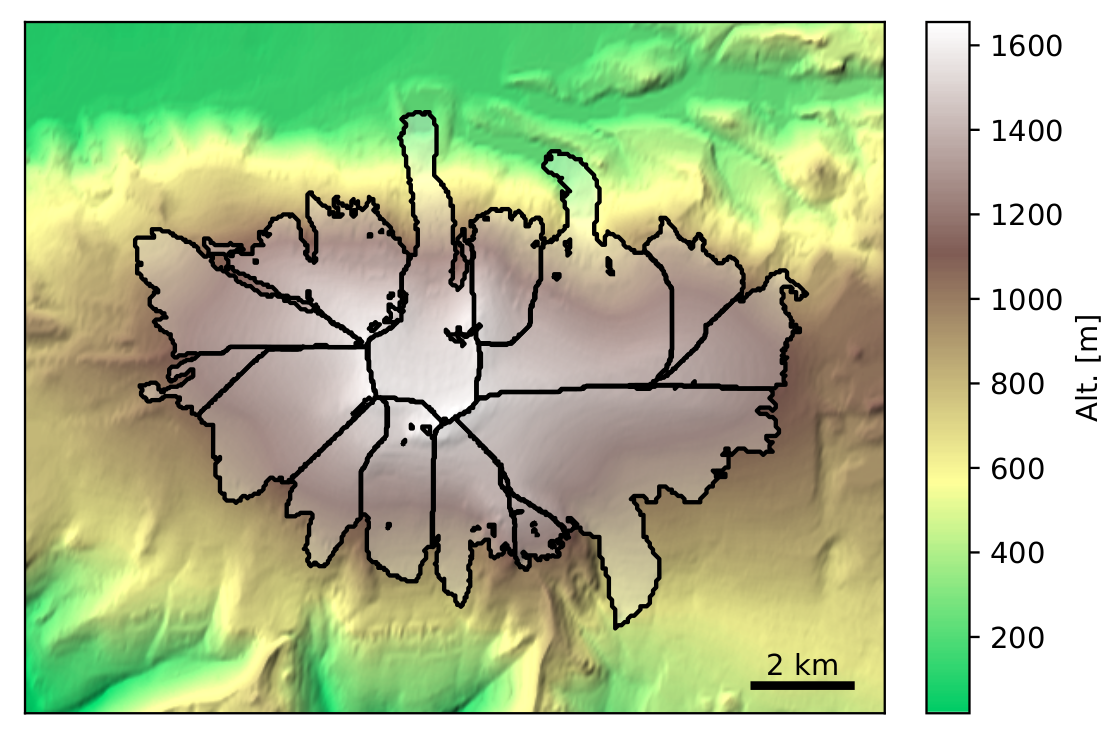
\includegraphics[width=0.7\linewidth]{\figs/iceland.png}
\caption{Glacier centric approach applied to the Eyjafjallajökull ice cap in Iceland.  Glacier outlines provided by the Randolph Glacier Inventory v6.0.}
\end{figure}

The glacier centric approach is used by most large-scale glacier models to date. Alternative strategies include global
gridded approaches \citep{Shannon2019}, where all glaciers in a model grid cell are added together and possibly
organized into elevation bins. Another approach is to handle entire glacier complexes as one single body of ice (“ice
caps”). This is physically consistent and feasible, but requires either distributed models of ice flow
\citep{Furst2017} (computationally expensive) or implies simplifications to the glacier geometry (so that all ice flows
downwards, \citep{Huss2012}).

The advantage of glacier centric models is their adherence to the de-facto standard inventory of glacier outlines:
the \href{https://www.glims.org/RGI/}{Randolph Glacier Inventory}. Any glacier can be selected and simulated, and the model
output can be compared to standard reference datasets such as length changes or surface mass balance data from
the \href{https://wgms.ch}{World Glacier Monitoring Service}. Various models can be compared on a glacier per glacier basis
or a combination of them. It is also computationally efficient, since models can focus on simulating the areas where
glaciers are really located. This may sound trivial, but glacier centric models can also make use of the glacier
location as a boundary condition, e.g. by excluding unrealistic solutions to the problem of computing mass balance or
inferring ice thickness, for example.

The disadvantage of glacier centric models is their questionable scientific validity in presence of glacier complexes
and ice divides (this problem can be mitigated by defining glacier complexes as one single entity, requiring other
strategies than currently standard in OGGM). A larger issue of glacier centric models is that they are focussed on
simulating glaciers that have been inventoried, i.e. they cannot retrieve past (or present) uncharted glaciers
\citep{Parkes2018}. For these reasons, they are not well adapted for studying glacier evolution in climates when
glaciers were widely different from today (e.g. the Last Glacial Maximum).


\subsection{Standard modelling workflow}

I briefly illustrate the OGGM workflow with an example application on the Tasman Glacier in New Zealand (see figure
below). Refer to the model documentation for more information.

\textbf{Preprocessing.}
The glacier outlines are extracted from a reference dataset (RGI)
and projected onto a local gridded map of the glacier (Fig.~\ref{fig:flow}a). Depending on the glacier location, a suitable source
for the topographical data is downloaded automatically and interpolated to the local grid. The spatial resolution of the
map depends on the size of the glacier.

\textbf{Flowlines.}
The glacier centerlines are computed using a geometrical routing algorithm
(Fig.~\ref{fig:flow}b), then filtered and slightly modified to become glacier “flowlines”
with a fixed grid spacing (Fig.~\ref{fig:flow}c).

\textbf{Catchment areas and widths.}
The geometrical widths along the flowlines are obtained by intersecting the normals at each grid point with the glacier
outlines and the tributaries’ catchment areas. Each tributary and the main flowline has a catchment area, which is then
used to correct the geometrical widths so that the flowline representation of the glacier is in close accordance with
the actual altitude-area distribution of the glacier (Fig.~\ref{fig:flow}d).

\textbf{Climate data and mass balance.}
Gridded climate data (monthly temperature and precipitation) are interpolated to the glacier location and corrected for
the altitude at each flowline’s grid point. A calibrated mass balance model is used to compute the mass balance for the
past, and for projections based on GCM data.

\textbf{Ice thickness inversion.}
Using the mass balance data computed above and relying on mass-conservation considerations, an estimate of the ice flux
along each glacier grid point cross-section is computed by making assumptions about the shape of the cross-section.
Using the physics of ice flow and the shallow ice approximation, the model then computes the thickness of the glacier
along the flowlines and the total volume of the glacier (Fig.~\ref{fig:flow}e).

\textbf{Glacier evolution.}
A dynamical flowline model is used to simulate the advance and retreat of the glacier under preselected climate time
series. Here (Fig.~\ref{fig:flow}f), a 120-yrs long random climate sequence leads to a glacier advance.


\begin{figure}[h]
\centering
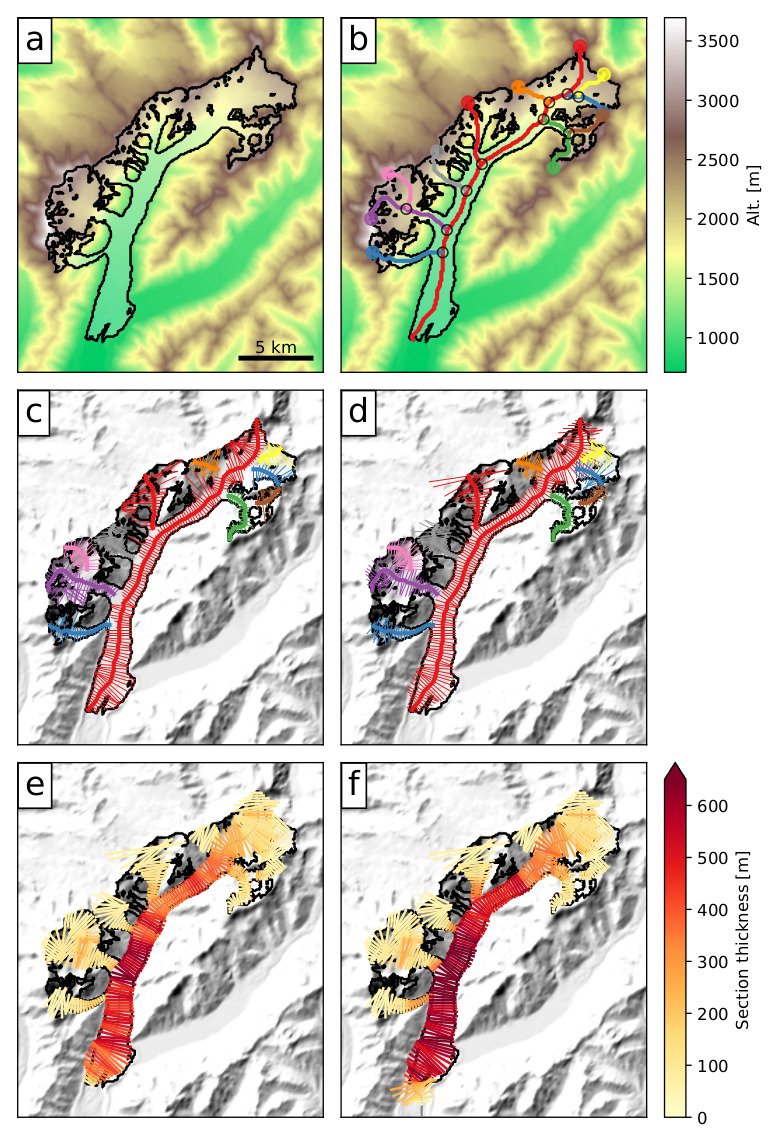
\includegraphics[width=0.700\linewidth]{\figs/ex_workflow.png}
\caption{Illustration of the OGGM standard workflow applied to Tasman Glacier.}
\label{fig:flow}
\end{figure}


\subsection{OGGM data structures and glacier directories}

The fundamental data structure used in OGGM is the so-called \textbf{Glacier Directory}. Glacier directories simply are
folders on disk which store the input and output data for a single glacier during a run. OGGM offers an object interface
to access and store these files programmatically.

This very simple idea is at the core of the OGGM workflow: actions to perform on glaciers (“tasks”, see below) are given
access to the data files via the glacier directory interface, read data they need from disk, and write back to it.

This design matches perfectly the “glacier centric” modelling strategy, and has many advantages:
\begin{itemize}
\item {} 
there is no practical difference between simulating one single, or many glaciers: all glacier directories are
independent of another.

\item {} 
data is persistent on disk: workflows can be interrupted and restarted from disk at no cost overhead. Workflows can
even be prepared on one computer and restarted from another computer (see example below).

\item {} 
“modularity” is achieved via data formats, not via programmatic interfaces: various ways to compute the flowlines (for
example) can co-exist if they agree on how a flowline is stored on disk.

\item {} 
multiprocessing is trivial: the same task can be run on many glaciers at once without having to share data across
processes, since everything is on disk and independant.

\end{itemize}

This persistence en disk has a few drawbacks as well:
\begin{itemize}
\item {} 
for the glacier directories to be independent, several data sources are duplicated: topography for example (each
glacier has its own subset of the original data, often overlapping with neighbors), or climate timeseries (the same
data from the same grid point is stored in various directories). This can lead to rather large data storage
requirements, but can be mitigated by deleting intermediate files.

\item {} 
since users can restart workflows from pre-processed states, the code that was used to produce them is often ignored
or might be older, etc. This can lead to silent bugs (for example mismatching model parameters between the preprocessing
and the simulations, leading to incorrect results). Because of this issue, we had to implement safeguards against such
mistakes where possible.

\item {} 
users can be confused by glacier directories. Since an OGGM program does not always read like linear “A to Z”
workflows (but for example “start from Q, then Q to Z”), mistakes like the ones described above can happen unnoticed.

\item {} 
it can make certain types of sensitivity experiments more difficult to implement, since users not only have to care
about variable names, but also data file names.

\end{itemize}

Here is an example of how glacier directories work in practice. The user indicates a repository from which
they want to fetch the data, and a list of glacier IDs they’d like to start from. The \mintinline{python}{init_glacier_directories}
performs the action of downloading and extracting these data locally.

\begin{figure}[H]
\captionsetup{singlelinecheck = false, justification=justified} 
\begin{minted}
[
]
{python}
from oggm import workflow, graphics

# Glaciers to simulate
rgi_ids = ['RGI60-11.01328', 'RGI60-11.00897']
# Where to fetch the pre-processed directories - this can be changed
server_url = 'https://cluster.klima.uni-bremen.de/~oggm/gdirs/'
experiment_url = 'oggm_v1.4/L3-L5_files/CRU/centerlines/qc3/pcp2.5/no_match'
base_url = server_url + experiment_url
# Fetch them
gdirs = workflow.init_glacier_directories(rgi_ids, from_prepro_level=3, 
                                          prepro_base_url=base_url)
# Plot the ice thickness inversion results
graphics.plot_inversion(gdirs[0])
\end{minted}
\vspace{10mm}
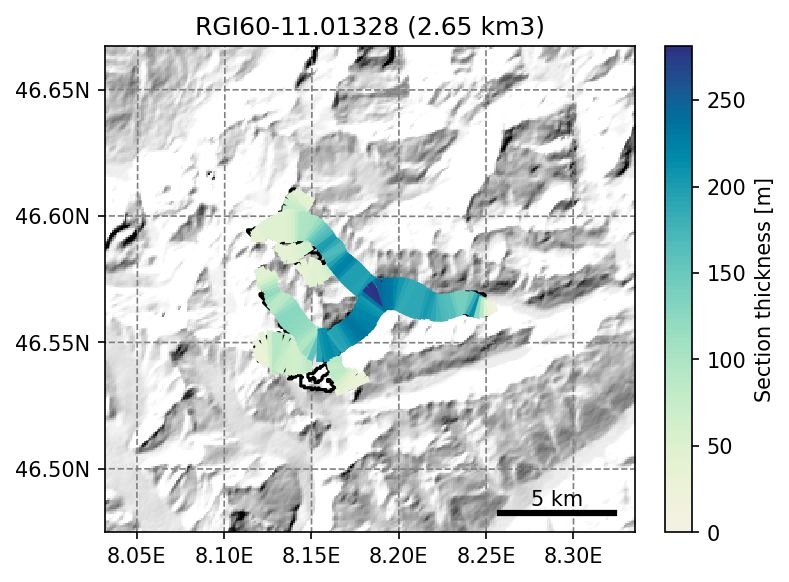
\includegraphics[width=0.600\linewidth]{\figs/unteraar_demo.png}
\caption{Example of the glacier directory workflow}
\end{figure}

See also the documentation page for \href{https://docs.oggm.org/en/stable/input-data.html}{OGGM-Shop}
for more examples of the kind of data that can be added to glacier directories.


\subsection{OGGM tasks}

Tasks in OGGM are actions to perform on one single glacier (“entity tasks”) or several of them (“global tasks”). Tasks
have a special meaning in the OGGM workflow and are applied as such:

\begin{figure}[H]
\begin{minted}
[
]
{python}
# Initialize glacier dir
from oggm import workflow, tasks

ectories
gdirs = workflow.init_glacier_directories(rgi_ids)

# Define the list of tasks
task_list = [
    tasks.define_glacier_region,
    tasks.glacier_masks,
    tasks.compute_centerlines,
    tasks.catchment_area,
    tasks.catchment_width_geom,
]

# Apply them sequentially
for task in task_list:
    workflow.execute_entity_task(task, gdirs)
\end{minted}
\end{figure}


\mintinline{python}{exectute_entity_task} will apply the given task to a list of glaciers. If multiprocessing is switched on, all glaciers
will be processed in parallel, making full use of all available processors. Here we apply the default tasks with default
settings, but parameters can be changed via global settings or function arguments.

Depending on the desired set-up, tasks can be replaced by others (e.g. the centerlines tasks can be replaced by other
algorithms) or omitted (for example, users can choose whether a quality check filter should be applied to the climate
timeseries or not).


\begin{figure}[h]
\centering
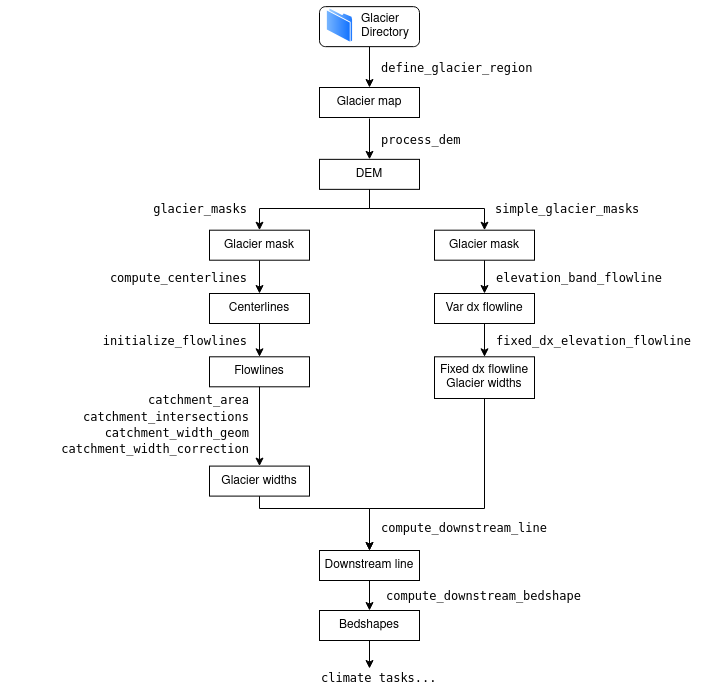
\includegraphics[width=0.700\linewidth]{\figs/flowchart_flowlines.png}
\caption{Example flowchart illustrating how OGGM implemented support for two kinds
of flowline representations for a glacier: centerlines on the left (OGGM’s default)
and binned elevation bands flowlines on the right (after \citet{Huss2012}).}
\end{figure}

\subsection{Take home messages}

The purpose of this rather technical description was to convey the general design of the model around the concept of a
list of tasks to be applied to glacier entities and that store their output in glacier directories on disk. Note that
except for their names and the objects they are referring to (glaciers), these “building blocks” are largely
agnostic to the kind of tasks that have to be applied, and I deliberately did not provide any modelling detail here.

This is important, because I believe that the OGGM project should not be considered by looking only at the physics
choices we’ve made for each of these tasks or their default parameters. OGGM should also be evaluated for the new
developments its structure can allow. OGGM does not enforce a particular modelling strategy beyond the constraints
defined above: in summary, complying models do need to follow the glacier directory approach (otherwise OGGM will be of
very little use for them). If new modelling groups develop ideas based on a glacier centric approach, they can make use
of OGGM’s building blocks and add their own, provided that they comply with this “OGGM way of doing things”.

By doing so, external projects based on OGGM will then benefit from all future developments in OGGM, and the other way
around: OGGM can then use and apply these external modules. If desired, external projects can also benefit from the
suite of modern open development tools that OGGM provides. I describe them below.


\section{Open development practices}

OGGM development has been strongly inspired by practices which have become a standard in the software development
community, but that are (unfortunately) not yet well known in the scientific community.

Like the vast majority of today’s software, OGGM’s development is done under a version control system
called \href{https://git-scm.com/}{git}. The OGGM repository is hosted on \href{https://github.com/OGGM/oggm}{github}, enabling
many of the tools described below.


\subsection{Code review}

Very much like peer-review, open development practices based on git enable code review. Open code review has many
advantages:
\begin{itemize}
\item {} 
it gives model developers the opportunity to discuss changes alongside the code rather than per email

\item {} 
it improves code quality, since more than one person can look at the code

\item {} 
it gives an opportunity to model users to follow changes in the model even if they are not actively participating

\item {} 
code changes and associated comments over time are stored online for later reference

\end{itemize}


\begin{figure}[h]
\centering
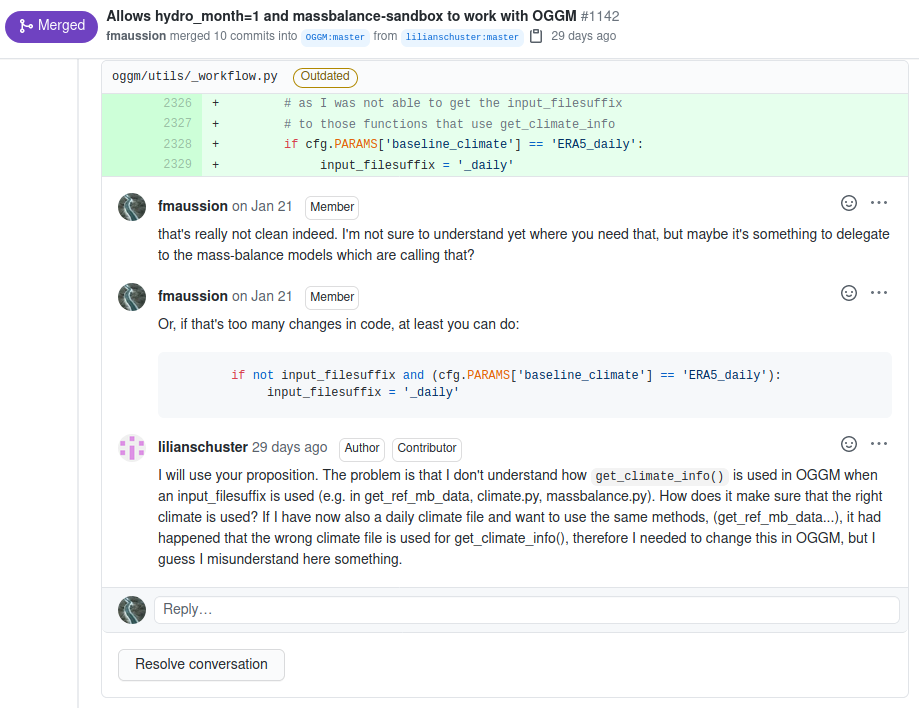
\includegraphics[width=0.900\linewidth]{\figs/pr.png}
\caption{Example of code review in a recent “\href{https://github.com/OGGM/oggm/pull/1142}{pull-request}”.}
\end{figure}

Ideally, all code submissions to OGGM should be peer-reviewed. In practice, however, only the contributions from others
than me are reviewed (by me). I’ll discuss this problem in more length below.


\subsection{Testing strategy}

OGGM enforces a strict code testing strategy: all additions to the code must be supplemented by appropriate tests. The
tests have the purpose to check that the code (i) can be executed without errors and (ii) works as expected. These tests
are an integral part of the codebase, and all of them are run each time a new code addition is suggested (a process
called \href{https://en.wikipedia.org/wiki/Continuous\_integration\#Run\_tests\_in\_CI}{continuous integration}), hereby
avoiding “regressions” as much as possible (when a change in one part of the code affects another in non-predictable
ways).

\begin{figure}[h]
\centering
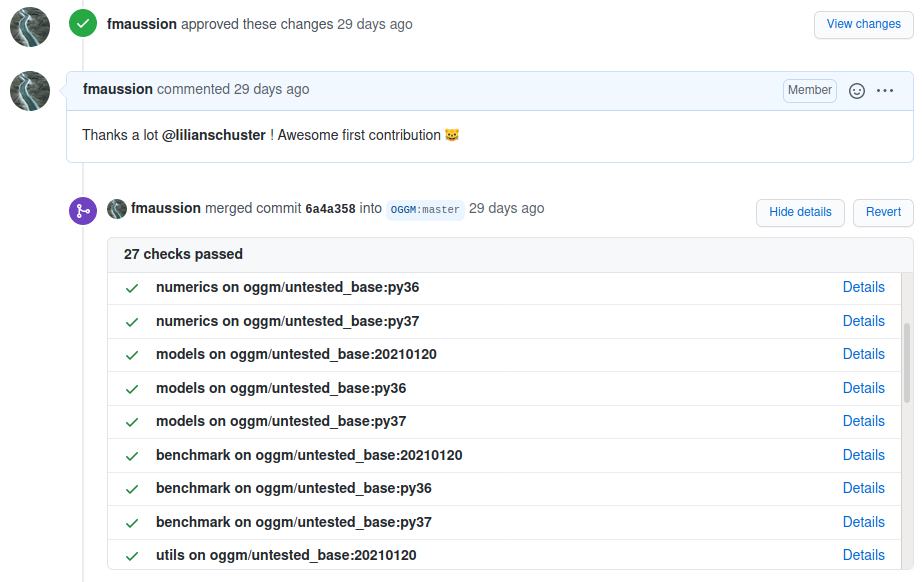
\includegraphics[width=0.700\linewidth]{\figs/tests.png}
\caption{Example of automated testing in a recent “\href{https://github.com/OGGM/oggm/pull/1142}{pull-request}”.}
\end{figure}


\subsection{Online documentation and tutorials}

Making code available is, by far, not enough to make code accessible. As of today, the OGGM codebase contains several
thousands of lines of code, making it very difficult for anyone new to the project to understand the model’s structure
just by reading the code.

Lack of code documentation (and the high cost of writing documentation) is probably one of the main obstacles towards
more open code sharing practices, as many scientists do not feel comfortable to share undocumented code. OGGM is no
exception (I always feel there could be better documentation for almost everything), but thanks to a suite of great
open-source tools, writing documentation for OGGM can also be rewarding. Writing documentation is also a very good way
to engage the community of users towards OGGM’s development, since contributing to the documentation can feel easier
than contributing to the code.

OGGM’s documentation relies on three main elements:
\begin{enumerate}

\item {} 
The project website (\href{https://oggm.org}{https://oggm.org}) for general, non code related project communication and blog posts.

\item {} 
The technical documentation (\href{https://docs.oggm.org}{https://docs.oggm.org}) to document model physics, model structure, and function calls
definitions.

\item {} 
The tutorials (\href{https://oggm.org/tutorials}{https://oggm.org/tutorials}) with hands-on model applications in various use cases.

\end{enumerate}

The project website is built using \href{https://jekyllrb.com/}{jekyll}, a static site generator. It’s source code and
content is also open and stored \href{https://github.com/OGGM/oggm.github.io}{on github}.

The technical documentation is built using \href{https://www.sphinx-doc.org}{sphinx} and is hosted
on \href{https://readthedocs.org/}{readthedocs}. Its content is stored alongside the code on the main repository.

The tutorials are written with \href{https://en.wikipedia.org/wiki/Project\_Jupyter\#Jupyter\_Notebook}{Jupyter Notebooks} and
rendered online with \href{https://jupyterbook.org}{Jupyter-Book}. The notebook interface allows sharing text and formulas
alongside the code, making them particularly adapted for tutorials. In addition, tutorials can be run and explored
interactively thanks to \href{https://mybinder.org}{MyBinder}. This is a great tool to engage new users, since they can try
the model online before going the struggle of installing it.


\subsection{Reproducibility}

OGGM attempts to make results obtained with the
model \href{https://en.wikipedia.org/wiki/Reproducibility\#Reproducible\_research}{reproducible} as far as possible. To do so,
the OGGM stable versions are stored with a DOI on \href{https://zenodo.org/record/4546676}{Zenodo}, and authors
are \href{https://docs.oggm.org/en/stable/citing-oggm.html}{encouraged} to use and cite stable OGGM versions (we can also
store older versions on demand if necessary).

Furthermore, a central tool that we offer to ensure that OGGM results are reproducible no matter the machine it is
running on, or the version of software packages that are installed
are \href{https://docs.oggm.org/en/stable/practicalities.html\#singularity-and-docker-containers}{docker containers}.
Containers are like a “software capsule”: they contain everything that OGGM needs to run and can be executed by any
machine that has Docker installed.


\section{Challenges}

To my knowledge at the time of writing, OGGM has been used for at least 13 peer-reviewed publications (3 are in review)
and has been an important part of 3 completed PhD theses. We expect these numbers to grow in the future, with new
generations of students and new collaborations starting just now. Several other indicators are suggesting that the OGGM project is being used by other
research groups, such as the number of requests to join our discussion channels and to use OGGM-Hub.

The fact that the OGGM project is now expected to suit these various needs
(new users with various expectations about OGGM capabilities, PhD students and PostDocs under time pressure,
project deadlines, etc) comes with a number of challenges which I briefly describe here.


\subsection{Technical debt}

The OGGM code base has grown and continues to grow organically, at the pace at which new features are added to the
model. Future innovation will be slowed down and maybe even impeded by the so-called “technical debt”: code that works
but would need considerable refactoring to adapt to new ideas and to allow further development.

Accumulating technical debt also makes testing the software and ensuring the validity of its results more challenging.
Certain functions might have been written in the past to take into account situations which are no longer an issue
today, adding unnecessary complexity to the code.

This often needed refactoring (process of restructuring and modernizing existing computer code)
is not without costs: it takes considerable time, is not rewarded by traditional academic measures such as publications,
and needs to be carefully conducted in order not to introduce new bugs into the software. Perhaps even more
problematically: existing users who wrote code based on OGGM are very unwilling to update it to the new OGGM versions (I
know this from experience).

There is therefore a trade-off between breaking backwards compatibility (i.e. breaking existing code) and
innovating. Other models with fewer users, or lower standards in terms of code reusability (this is not always a bad thing),
may be more agile and quicker in innovating because no other people are relying on their code being stable.


\subsection{Software maintenance and entry level for new contributors}

A large part of routine software development maintenance currently relies on one or two main developers (myself, and an
IT technician in Bremen who is in charge of the technical aspects of the deployment of OGGM).
This work takes a lot of time (mainly because every new feature needs to be tested and documented), and my time is
limited. Therefore, the development process is slower than I’d like it to be.

As the software grows and increases in complexity, it becomes more difficult for new users to understand the model’s
structure and to apply it to their specific research problem. Furthermore, it makes it harder for new users to
envision a potential contribution to the code base. The typical model contributors (PhD students and post docs) are
employed on fixed-term contracts, causing a high turnover, making transmission of knowledge particularly difficult.

Finally, not all scientists are interested in writing reusable code, as is required when contributing to OGGM.
Very few have the time, energy, or interest to invest in the rather demanding field of scientific programming,
while staying on top of the other requirements of our job. I had the privilege to be given enough time to realize this
project over the course of several years, thanks to my stable employment at the university of Innsbruck. No other
traditional funding scheme in Austria would have allowed this kind of long haul development work.

The future of OGGM’s technical development and maintenance therefore strongly relies on funding agencies
acknowledging that open-source development work is an integral part of the scientific process. Employers should reward
open source work at the same level as scientific publications when considering applications.


\subsection{Innovation with OGGM}

I often ask myself the question of the role of OGGM in comparison to similar models in the geosciences.
Let’s take the atmospheric model \href{https://www.mmm.ucar.edu/weather-research-and-forecasting-model}{WRF}
as a prominent example. WRF is open-source, and its user base is obviously larger than OGGM by several orders of
magnitude. The reason is not only that WRF is an atmospheric model, and a much more mature and feature complete model.
I believe that a major reason is that users can take the model, learn how to use it (without knowing the internal
details of its functioning), and apply it to their research question with very few modifications (change of domain,
change of boundary conditions).

Attempting to make a parallel with OGGM will unravel some differences:

\begin{itemize}
\item {} 
For one, OGGM already simulates
all glaciers. I.e. “changing the domain” is not meaningful, unless the study attempts to simulate glaciers
differently, or analyse the data from a new perspective.

\item {} 
Second, since OGGM is highly parameterized, applying it blindly, without a specific awareness of its simplifications
and potential pitfalls, is not recommended.
This point is also valid for WRF, but I would argue that it is less problematic: thanks to the large
amount of available data for independent validation, users are able to check if their simulations are meaningful.
With a model like WRF, where the boundaries between calibration and validation data are fuzzier, it is difficult
for users to assess whether they apply the model correctly or not.

\item {} 
Finally, application of OGGM to a new research question almost inevitably leads to the development of extensions to
OGGM, or modifications of its internal code. This comes with the nature of the model: since the standard modelling of all
glaciers is possible “out-of-the box”, innovation can only come with active participation in the model development,
it’s capacity to deal with new boundary conditions, a new model parameterization, etc.

\end{itemize}

To summarize, and despite all our efforts to make OGGM user-friendly, I think that for the time being OGGM is
still a model “for modellers”, not yet ready for blind application. Because of the nature of the problems that
OGGM is trying to solve, it might never be “a model for users”, and remain “a model (or framework) for modellers”.
I think that this is something I’d be happy with, but it has implications for the people willing to learn how to apply
the model -- in particular in terms of required programming and glacier modelling skills.
\cleardoublepage

\newcommand{\papertext}{Paper 01: Model description}

\section*{\papertext}
\addcontentsline{toc}{section}{\protect\numberline{}\papertext}%
\label{paper_01}

\vspace{0.5cm}

\begin{singlespace}
\begin{hangparas}{1em}{1}
\textbf{Maussion, F.}, Butenko, A., Champollion, N., Dusch, M., Eis, J., Fourteau, K., Gregor, P., Jarosch, A. H., Landmann, J., Oesterle, F., Recinos, B., Rothenpieler, T., Vlug, A., Wild, C. T. and Marzeion, B.: The Open Global Glacier Model (OGGM) v1.1, Geosci. Model Dev., 12(3), 909–931, \\
\href{https://doi.org/10.5194/gmd-12-909-2019}{doi:10.5194/gmd-12-909-2019}, 2019.
\end{hangparas}
\end{singlespace}

\vspace{0.5cm}


%\includepdf[pages=-,openright]{./papers/paper_01.pdf}



\chapter{Ice thickness estimation}
\label{chap3}

\cleardoublepage

\renewcommand{\papertext}{Paper 02: How accurate are estimates of glacier ice thickness? Results from ITMIX, the Ice Thickness Models Intercomparison eXperiment}

\section*{\papertext}
\addcontentsline{toc}{section}{\protect\numberline{}\papertext}%
\label{paper_02}

\vspace{0.5cm}

\begin{singlespace}
\begin{hangparas}{1em}{1}
Farinotti, D., Brinkerhoff, D. J., Clarke, G. K. C., Fürst, J. J., Frey, H., Gantayat, P., Gillet-Chaulet, F., Girard, C., Huss, M., Leclercq, P. W., Linsbauer, A., Machguth, H., Martin, C., \textbf{Maussion, F.}, Morlighem, M., Mosbeux, C., Pandit, A., Portmann, A., Rabatel, A., Ramsankaran, R., Reerink, T. J., Sanchez, O., Stentoft, P. A., Singh Kumari, S., van Pelt, W. J. J., Anderson, B., Benham, T., Binder, D., Dowdeswell, J. A., Fischer, A., Helfricht, K., Kutuzov, S., Lavrentiev, I., McNabb, R., Gudmundsson, G. H., Li, H. and Andreassen, L. M.: How accurate are estimates of glacier ice thickness? Results from ITMIX, the Ice Thickness Models Intercomparison eXperiment, Cryosph., 11(2), 949--970, \href{https://doi.org/10.5194/tc-11-949-2017}{doi:10.5194/tc-11-949-2017}, 2017.
\end{hangparas}
\end{singlespace}

\vspace{0.5cm}

This paper is the result of an international working group of the International Association of
Cryospheric Sciences (IACS): the working group on \href{https://cryosphericsciences.org/activities/ice-thickness}{Glacier ice thickness estimation}  (2014--2019),
of which I was a member. The group activities led to several major publications, two of them are presented in
this thesis.

The first collaborative effort of the working group was the “Ice Thickness Models Intercomparison eXperiment (ITMIX)”,
phase 1. It was the first coordinated assessment of the individual performance of independent methods able to infer
glacier ice thickness from characteristics of the surface. A set of 17 different models were used to estimate the ice
thickness “blindly”, i.e. without using any observations for model calibration or tuning.

This publication is a milestone in the field of glacier ice thickness estimation. Cited more than 110 times to date (
Google Scholar), it laid the ground for a wealth of follow-up studies, leading several research groups (including mine)
to increase efforts in developing new methods to estimate the volume of glaciers. Indeed, we showed that the
disagreement between models themselves and between models and observations can be very large (up to several times the
observed ice thickness). Ensemble approaches may reduce model errors, but no model consistently outperformed the others.
A few models were favorably listed for their ability to robustly simulate many glaciers with a reasonable accuracy (e.g.
OGGM, Huss), or for their high accuracy on fewer glaciers (e.g. Brinkerhoff-v1),

My contribution to this paper was the participation in several meetings that helped to shape the experimental design,
and I participated with a model contribution. OGGM was ranked among the best models able to estimate ice thickness from
limited information (i.e. able to compute many glaciers). I also contributed to the analysis of the
results, and played a minor role in the writing of the paper.


\href{https://doi.org/10.5194/tc-11-949-2017}{Link to the paper} (open access).


%\includepdf[pages=-,openright]{./papers/paper_02.pdf}



\chapter{Glacier mass balance}
\label{chap4}

\chapter{Past and future glacier change}
\label{chap5}

\chapter{OGGM-Edu}
\label{chap6}

\chapter{Conclusions}
\label{chap7}

The OGGM global glacier modelling framework is now well established in the landscape of
glacier models. It is the only global-scale model that is open source, which has
attracted many users and contributors from external institutions. It forms the basis of this thesis,
several research publications and PhD theses, and is the backbone of current research projects and
proposals.

Very few global models reach a similar level of physical complexity. At present, only the model by
\citet{Huss2015} and \citet{Zekollari2019}  aims for similar complexity and has
been a driver for many advances in global scale glaciology in recent years. A new model \citep[PyGEM,][]{Rounce2020}
became open source recently: focussed on simulating the surface mass balance and its uncertainty with Bayesian
methods, PyGEM is arguably one of the best mass balance models available. Thanks to a recent collaboration, PyGEM is now
relying on OGGM for its pre-processing and ice dynamics components, making it the first external application
of OGGM’s “framework” structure: PyGEM remains independent while still using some elements
of the OGGM workflow, opening the way for future model intercomparison studies.

Additional unpublished models are currently in development (see below), but OGGM is still probably one of the most
modern and complete global glacier models available. It is unprecedented in terms of open development, modular
structure and testing practices.

This alone won’t guarantee that OGGM continues to be useful in the future.

In the following, I briefly discuss my personal opinions about the directions that the OGGM project might follow.
What other research groups will do with OGGM is not under my control, and I’m sure that I’ll be up for some surprises.

\textbf{Surface mass balance and model calibration}

One of the major recent advances for global glacier studies has been the publication of geodetic mass balance estimates at the
regional and (very soon) global scale. We now have a mass balance estimate for almost every single glacier of the world.
This is a tremendous opportunity for glacier models, opening new avenues of research.
It will raise very important questions with respect to model calibration and validation (since all models will
be matching the same reference products, how to compare their performance?), and with respect to the added value of
physical parameterisations (since out-of-sample validation will be more difficult, how do we estimate added value?).

We are now preparing OGGM to ingest these new products. In a recently started PhD project
(Lilian Schuster), we attempt to address the question of the added value of physical processes in mass balance models
by implementing a suite of parameterizations of varying complexity. We will include combinations of surface processes
(refreezing, snow cover properties, debris cover…) and study the impact of these model physics on glacier projections.
This project will provide a new generation of mass balance models to the OGGM framework and, hopefully, open the door for an
automated and systematic model uncertainty quantification.

\textbf{Ice dynamics: distributed and flowline approaches}

A new generation of models currently in development are aiming for distributed (2D/3D) modelling of surface mass balance
and ice dynamics. I am aware of at least three independent efforts: Johannes
Fürst (EU Starting grant at Universität Erlangen), Harry Zekollary (TU Delft / ETH Zürich), and Bert Wouters / Jordi Bolibar
(Universiteit Utrecht). Distributed approaches are more elegant, less parameterized, and physically more sensible than
the current approach used by OGGM. I welcome these new developments, and the OGGM framework will
be ready to provide boundary conditions for these models if they need them (for example, OGGM will be used to provide
the glacier attributes delivered with the future version of the RGI, and we will make sure to address the needs of these
new projects as well).

I, personally, still believe that OGGM’s flowline model will continue to be useful in the future. Included in OGGM
only a few years ago, it allowed the representation of much more realistic dynamic feedbacks than parameterized or
“delta h” approaches. This will certainly be the subject of scientific debate in the near future,
but I believe that the quality of our observations, boundary conditions, and estimates of ice thickness will not yet
allow to use the full potential of distributed modelling (at least not at the global scale), and the use of distributed
models will come with its own set of challenges and uncertainties.

Personally (and I might be mistaken), I am investing most of my thoughts and energy on improving OGGM as it is now,
in particular in the domain of statistical methods for uncertainty estimation. The Bayesian model ensemble strategies
and the inverse models we are planning to use will be very hungry in computational resources, and the efficiency and
robustness of the flowline model will be a central requirement for these new applications.
Furthermore, I also think that one of the largest remaining challenges for global models (frontal ablation)
will be more likely to be tackled by flowline than distributed models, at least in a first step.

\textbf{Frontal ablation}

46\% of the area of the world’s mountain glaciers eventually flows directly into water (marine-, shelf-, and
lake-terminating glaciers). As discussed in this thesis, frontal ablation strongly impacts the dynamic response of
glaciers, and raises new challenges for model calibration and ice thickness estimation.
I believe that frontal ablation is the most important source of biases in current global-scale glacie change projections,
and a problem that the glacier modelling community needs to address urgently.

It is a very difficult problem, requiring collaborations with ice-sheet and ocean experts, modelling  and remote
sensing specialists. Over the past few years, we have opened the door to such collaborations by implementing parameterizations
in the framework. Because of lack of testing in real-world global applications they are, however, switched off
per default at the moment. With these first building blocks in place, we hope that OGGM will
be useful to the research groups that are interested in such an endeavor.

\textbf{Inverse methods for ice thickness estimation}

The mass-conservation method used by OGGM to estimate the ice thickness relies on an important and problematic
assumption: that glaciers are in dynamical equilibrium with a given mass-balance profile. To release this
assumption, I have worked with two master students on a completely new approach based on cost optimisation:
\href{https://github.com/OGGM/combine}{COMBINE} (COst Minimization Bed INvErsion model for glaciers and ice caps).

This new approach relies on the OGGM distributed or flowline model as a forward operator, and uses automatic
differentiation to iteratively minimize the mismatch with observable variables such as surface height or
ice thickness observations. COMBINE will allow to ingest much more information into the inversion process,
such as past climate data and past glacier outlines, hereby releasing the equilibrium assumption. It will
also lead to improved present day glacier states and reduce the “initialisation shock” that happens in the
first few years of an OGGM simulation.

A research project proposal based on COMBINE is currently in the making.





%\input{./chapters/chapter1}
%\input{./chapters/chapter2}
%\input{./chapters/chapter3}
%\input{./chapters/chapter4}
%\input{./chapters/chapter5}
%\input{./chapters/chapter6}
%\input{./chapters/chapter7}
%\input{./chapters/chapter8}

%\input{./papers/paper1}
%\input{./papers/paper2}
%\input{./papers/paper3}
%\input{./papers/paper4}
%\input{./papers/paper5}

\cleardoublepage\phantomsection
\bibliographystyle{copernicus}
\bibliography{../habil/references}

\end{document}
